% Gemini theme
% https://github.com/anishathalye/gemini

\documentclass[final]{beamer}

% ====================
% Packages
% ====================

\usepackage[T1]{fontenc}
\usepackage[default]{raleway}
\usepackage{fontspec}
% \newfontfamily\Raleway[%
%   Path = /Library/Fonts/ ,
%   UprightFont = ,
%   BoldFont = -Bold ,
%   ItalicFont = -Oblique ,
%   Extension = .ttf
% ]{Raleway}
\usepackage{lmodern}
\usepackage[size=custom,width=120,height=72,scale=1.0]{beamerposter}
\usetheme{gemini}
\usecolortheme{gemini}
\usepackage{graphicx}
\usepackage{booktabs}
\usepackage{tikz}
\usepackage{pgfplots}
\pgfplotsset{compat=1.14}
\usepackage{anyfontsize}

% ====================
% Lengths
% ====================

% If you have N columns, choose \sepwidth and \colwidth such that
% (N+1)*\sepwidth + N*\colwidth = \paperwidth
\newlength{\sepwidth}
\newlength{\colwidth}
\setlength{\sepwidth}{0.025\paperwidth}
\setlength{\colwidth}{0.3\paperwidth}

\newcommand{\separatorcolumn}{\begin{column}{\sepwidth}\end{column}}

% ====================
% Title
% ====================

\title{Developing an Interactive Agent for Blind and Visually Impaired People}

\author{Vincent Stragier \inst{1} \and Omar Seddati \inst{1} \and Thierry Dutoit \inst{1}}

% \institute[shortinst]{\inst{1} Some Institute \samelineand \inst{2} Another Institute}
\institute[shortinst]{\inst{1} Numediart Institute, ISIA Lab, Faculty of Engineering — University of Mons — Boulevard Dolez 31, 7000 Mons, Hainaut, Belgium}

% ====================
% Footer (optional)
% ====================

\footercontent{
  % \href{https://www.example.com}{https://www.example.com}
  \hfill
  ACM International Conference on Interactive Media Experiences (IMX '23), June 12--15, 2023, Nantes, France 
  \hfill
  \href{mailto:vincent.stragier@umons.ac.be}{vincent.stragier@umons.ac.be}}
% (can be left out to remove footer)

% ====================
% Logo (optional)
% ====================

% use this to include logos on the left and/or right side of the header:
\logoright{
\includegraphics[height=5cm]{logos/logos_r.pdf}}
\logoleft{
\includegraphics[height=5cm]{logos/logos_l.pdf}}

% ====================
% Body
% ====================

\begin{document}

\begin{frame}[t]
  \begin{columns}[t]
    \separatorcolumn

    \begin{column}{\colwidth}

      \begin{block}{Motivation}
        In Belgium, at least 1~\% of the population suffers from visual impairment and about 0.1~\% is legally blind. These numbers are expected to raise due to the ageing of the population.

        Therefore, it is important to develop new assistive tools to help these people in their daily life. Existing tools are often expensive and not always user-friendly. Better solutions like the Be My Eyes\cite{IntroducingOurVirtual2023} app exist, but they are not always adapted to the needs of the users (resource intensive, no offline mode). For intense, the Virtual Volonteer of Be My Eyes is using GPT-4\cite{GPT42023}, which is a very resource intensive system.

        In this context, we propose to develop an interactive agent using a hybrid and multimodal approach.
      \end{block}

      \begin{block}{A modular approach}
        One of the goal of this project is to be able to implement assistive tools as modules in the systems. Through discussion with experts and users, a set of potential modules has been identified.

        The modules to implement are: face recognition, age and sex recognition, emotion recognition, color recognition, optical character recognition (OCR), money recognition, environment recognition, object recognition, navigation.
      \end{block}

      \begin{alertblock}{Generic architecture of an interactive agent}

        A typical (vocal) interactive agent is composed of on microphone and a speaker as its main inputs and output devices. The main part of the agent can be divided into five modules: speech recognition, natural language understanding, dialogue management, natural language generation, and speech synthesis. Furthermore, the agent can be interfaced with the physical world through digital systems.
        \begin{figure}[ht]
          \centering
          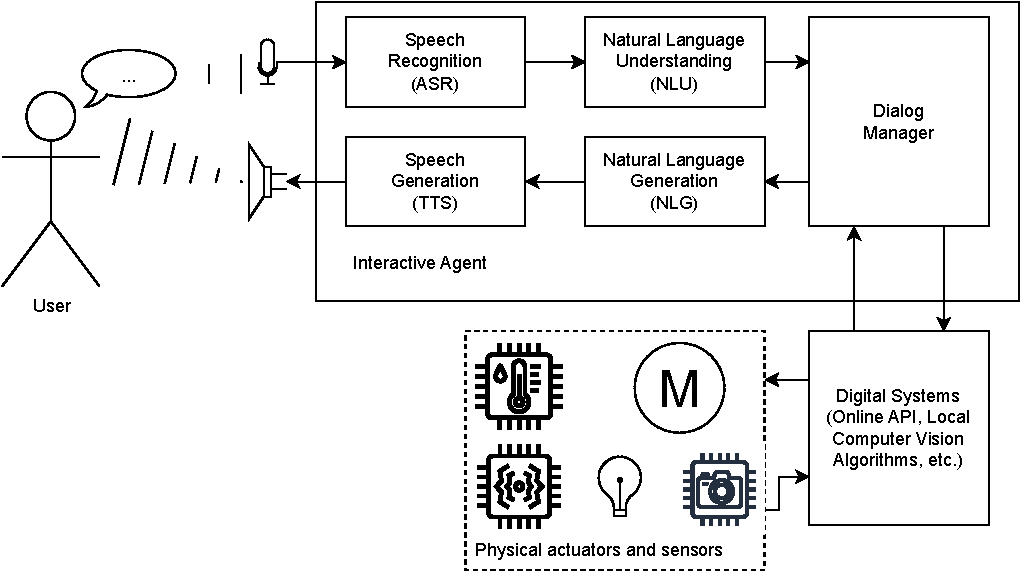
\includegraphics[width=0.8\linewidth]{figures/schematics-generic_architecture.drawio.pdf}
          \caption{Generic architecture of a conversational interface\cite{lugrinHandbookSociallyInteractive2021}.\label{fig:architecture_conversational_interface}}
        \end{figure}

      \end{alertblock}

    \end{column}

    \separatorcolumn

    \begin{column}{\colwidth}

      \begin{block}{An hybrid approach}
        Former interactive agent used NLP techniques, intent detection, named entity recognition, grammars, etc.

        Newer techniques rely on deep learning, or more specifically, on large language models.

        We propose to build a system that combine both classic NLP techniques to handle the typical user request and a fallback system based on a large language model to handle the more exotic requests.

        At the moment, we are developing a web application in order to test this system.
        \begin{figure}[ht]
          \centering
          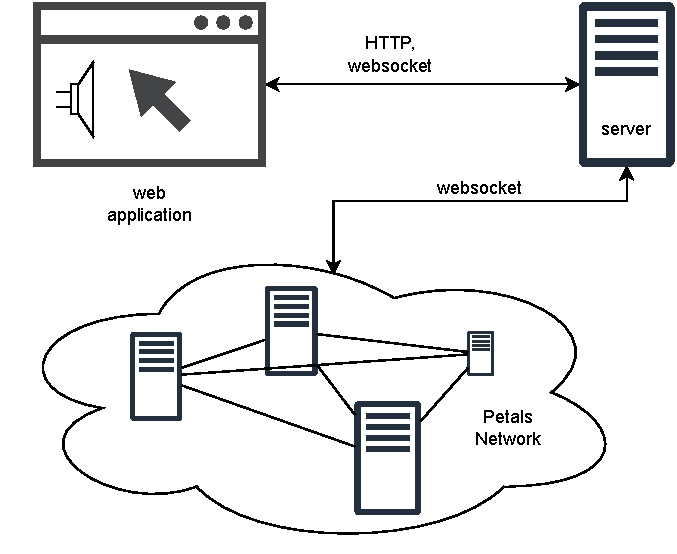
\includegraphics[width=0.5\linewidth]{figures/schematics-interactive_agent.drawio.pdf}
          \caption{Abstractive technical view of the prototype.\label{fig:abstractive_view_interface}}
        \end{figure}
      \end{block}

      \begin{block}{Integration of modules}
        One module of interest for social reasons is the facial recognition system.

        The biggest challenge in this module is to be accurate and near real-time while being privacy-preserving and resource efficient.

        Retinaface\cite{dengRetinaFaceSinglestageDense2019} (face detection) and Facenet\cite{jekelClassifyingOnlineDating2018}  may be the best candidates for this task.

        Last but not least, we plan to use a local database to store the faces and the faces embeddings.

        \begin{figure}[!ht]
          \centering
          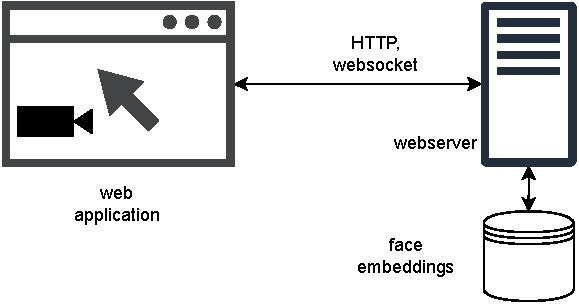
\includegraphics[width=0.5\linewidth]{figures/schematics-facial_recognition_system.drawio.pdf}
          \caption{Technical view of the prototype of facial recognition system.\label{fig:facial_recognition_technical_view}}
        \end{figure}
      \end{block}

    \end{column}

    \separatorcolumn

    \begin{column}{\colwidth}

      % \begin{exampleblock}{A highlighted block containing some math}
      %   \heading{A heading inside a block}

      %   \heading{Another heading inside a block}
      % \end{exampleblock}
      \begin{exampleblock}{}
        \begin{figure}[!ht]
          \centering
          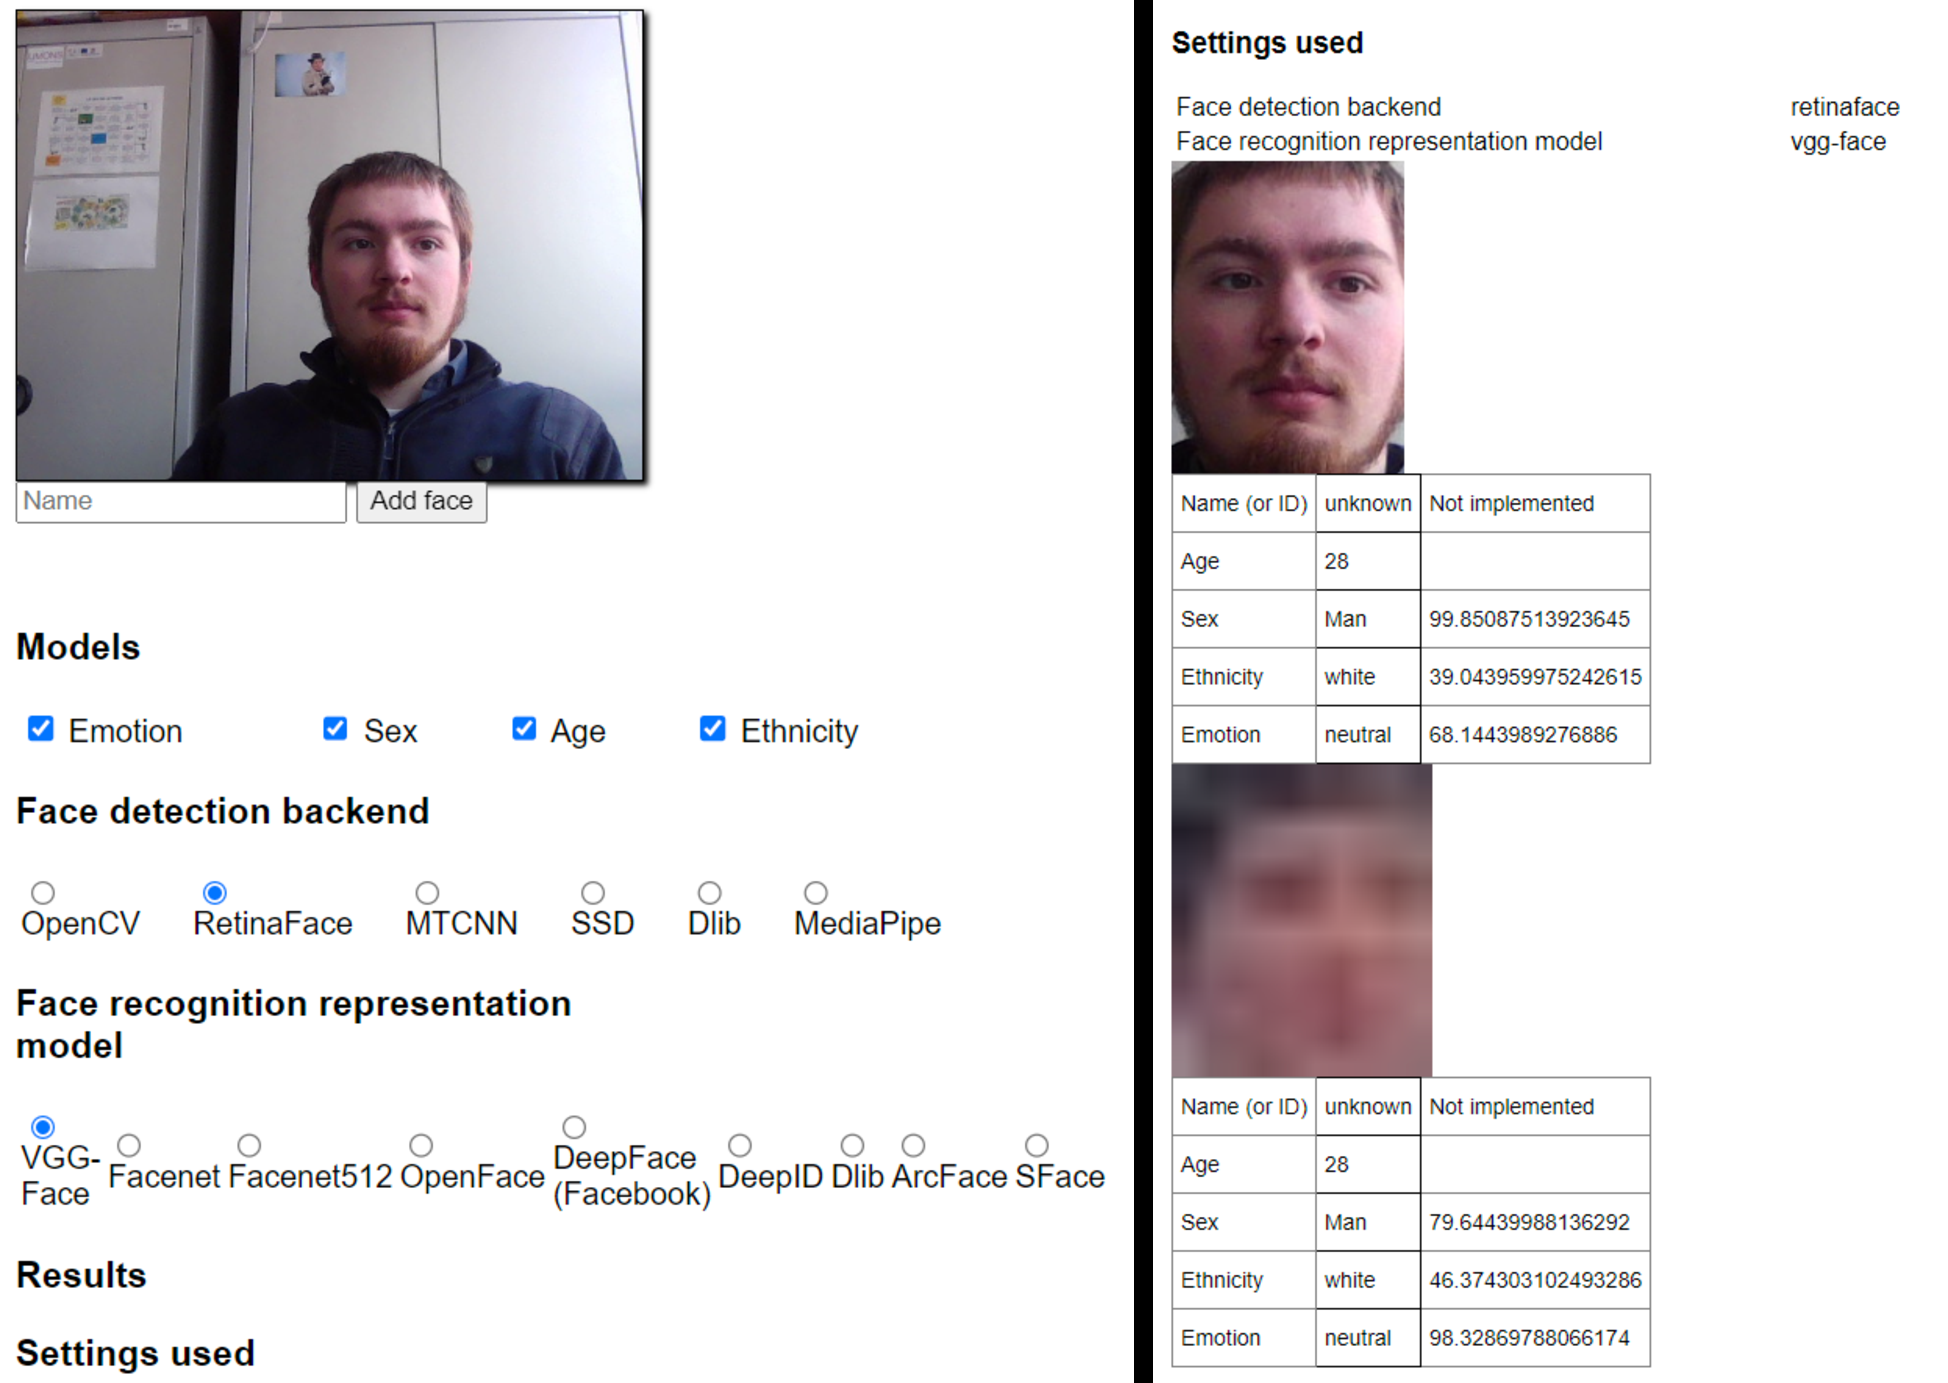
\includegraphics[width=0.65\linewidth]{figures/proto_interface.pdf}
          \caption{Two screenshots of the prototype's interface. On the left side, a live view of the camera is showed and various settings are available. On the right, two persons have been detected, and the interface shows the results of all the selected models.\label{fig:facial_recognition_interface}}
        \end{figure}
      \end{exampleblock}

      \begin{block}{Acknowledgements}

        \footnotesize{This research is funded by the European Regional Development Fund (ERDF). Vincent Stragier is funded through a PhD grant from the Œuvre fédérale Les Amis des Aveugles et Malvoyants ASBL- The Friends of the Blind and Visually Impaired Federal Charity-, Ghlin, Belgium.}

      \end{block}

      \begin{block}{References}

        % \nocite{*}
        \footnotesize{\bibliographystyle{plain}\bibliography{thesis_sources}}

      \end{block}

    \end{column}

    \separatorcolumn
  \end{columns}
\end{frame}

\end{document}
